% NeurIPS Poster — Sparse Neural Connectivity Recovery
% Compile: tectonic poster.tex
\documentclass[final]{beamer}
\usepackage[orientation=landscape,size=a1,scale=1.2]{beamerposter}
\usepackage{graphicx}
\usepackage{amsmath,amssymb,amsfonts}
\usepackage{booktabs}
\usepackage{array}
\usepackage{colortbl}
\usepackage{tikz}
\usepackage[most]{tcolorbox}

% ── Theme ──────────────────────────────────────────────────────────────────
\usetheme{default}
\setbeamertemplate{navigation symbols}{}
\setbeamertemplate{headline}{}
\setbeamertemplate{footline}{}

% Colors
\definecolor{neuripsblue}{HTML}{2E4057}
\definecolor{neuripsaccent}{HTML}{0077B6}
\definecolor{neuripsgray}{HTML}{F0F0F0}
\definecolor{neuripsgreen}{HTML}{2A9D8F}
\definecolor{neuripsred}{HTML}{E76F51}
\definecolor{boxbg}{HTML}{FAFAFA}

\setbeamercolor{block title}{fg=white,bg=neuripsblue}
\setbeamercolor{block body}{fg=black,bg=boxbg}
\setbeamercolor{title}{fg=neuripsblue}

% Box style
\tcbset{
  posterbox/.style={
    enhanced,
    colback=white,
    colframe=neuripsblue,
    boxrule=1.5pt,
    arc=4mm,
    left=8mm,right=8mm,top=6mm,bottom=6mm,
    fonttitle=\Large\bfseries\color{white},
    coltitle=white,
    colbacktitle=neuripsblue,
    attach boxed title to top left={xshift=6mm,yshift=-3mm},
    boxed title style={sharp corners,colback=neuripsblue}
  }
}

\begin{document}
\begin{frame}[t]

% ════════════════════════════════════════════════════════════════════════════
% TITLE BAR
% ════════════════════════════════════════════════════════════════════════════
\vspace{-1cm}
\begin{center}
{\fontsize{52}{58}\selectfont\bfseries\color{neuripsblue}%
Recovering Sparse Neural Connectivity from Partial Measurements}\\[12pt]
{\LARGE Quilee Simeon \hspace{1cm} Massachusetts Institute of Technology \hspace{1cm} \texttt{qsimeon@mit.edu}}
\end{center}
\vspace{0.3cm}

\begin{columns}[T]

% ════════════════════════════════════════════════════════════════════════════
% COLUMN 1 — The Problem + How We Solve It
% ════════════════════════════════════════════════════════════════════════════
\begin{column}{0.32\linewidth}

% ── The Question ──
\begin{tcolorbox}[posterbox,title=The Question]
\large
\textbf{How do you map a brain circuit's wiring when you can never see all the neurons at once?}

\vspace{4mm}
In small circuits (\textit{C.~elegans}, zebrafish, organoids), each recording session captures a different \emph{subset} of neurons. Different days $\to$ different views of the same circuit.

\vspace{4mm}
\centering
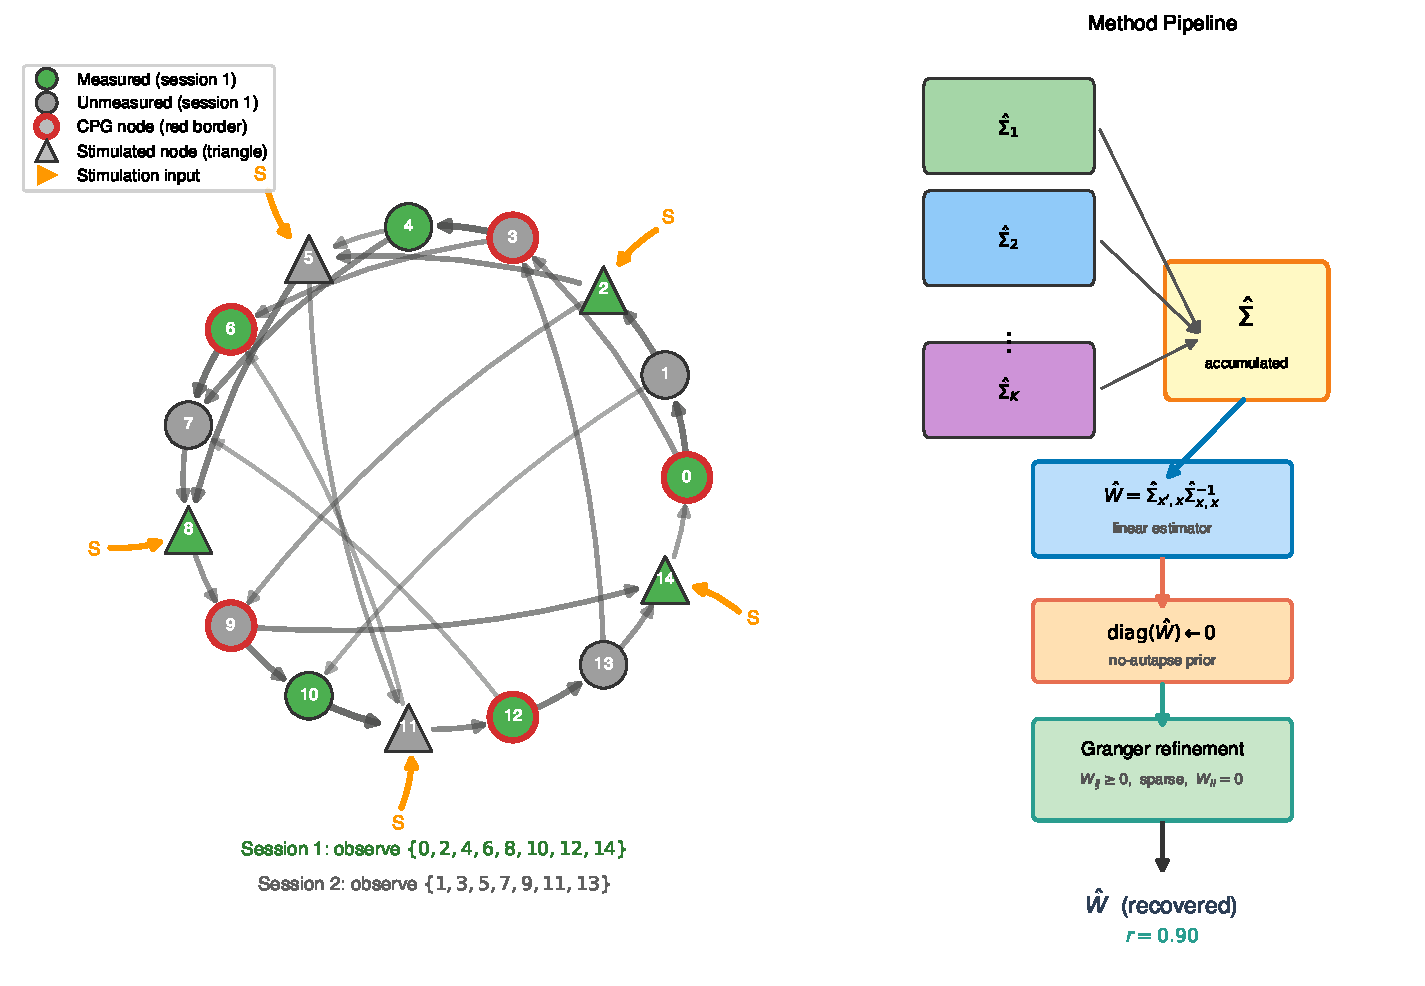
\includegraphics[width=0.92\linewidth]{figures/fig1_problem_schematic.pdf}
\end{tcolorbox}

\vspace{0.8cm}

% ── Our Approach ──
\begin{tcolorbox}[posterbox,title=Our Approach: Covariance Accumulation]
\large
\textbf{Whenever two neurons are co-observed}, their covariance tells you about the connection between them. Across $K{=}50$ sessions, you piece together the \textbf{full picture}.

\vspace{4mm}
Three steps:
\begin{itemize}\setlength{\itemsep}{3pt}
  \item[\color{neuripsaccent}\textbf{1.}] \textbf{Accumulate} pairwise covariances across sessions
  \item[\color{neuripsaccent}\textbf{2.}] \textbf{Estimate}: $\hat{W} = \hat{\Sigma}_{x_{t+1},x_t} \hat{\Sigma}_{x_t,x_t}^{-1}$, zero diagonal
  \item[\color{neuripsaccent}\textbf{3.}] \textbf{Refine} with biological constraints (sparsity, non-negativity)
\end{itemize}

\vspace{4mm}
Simple, closed-form, no deep learning required.
\end{tcolorbox}

\vspace{0.8cm}

% ── Headline Numbers ──
\begin{tcolorbox}[posterbox,title=Results at a Glance,colframe=neuripsaccent,colbacktitle=neuripsaccent]
\large
\begin{center}
\renewcommand{\arraystretch}{1.8}
\begin{tabular}{>{\bfseries\color{neuripsaccent}}l l}
  Weight correlation & $r = 0.96$ \\
  Improvement over chance & $84\%$ \\
  Best error & $0.050$ at $N{=}30$ \\
  Perfect edge recall & median $= 1.0$ \\
\end{tabular}
\end{center}
\end{tcolorbox}

\end{column}

% ════════════════════════════════════════════════════════════════════════════
% COLUMN 2 — What We Found
% ════════════════════════════════════════════════════════════════════════════
\begin{column}{0.32\linewidth}

% ── Granger refinement ──
\begin{tcolorbox}[posterbox,title=Recovery Quality]
\centering
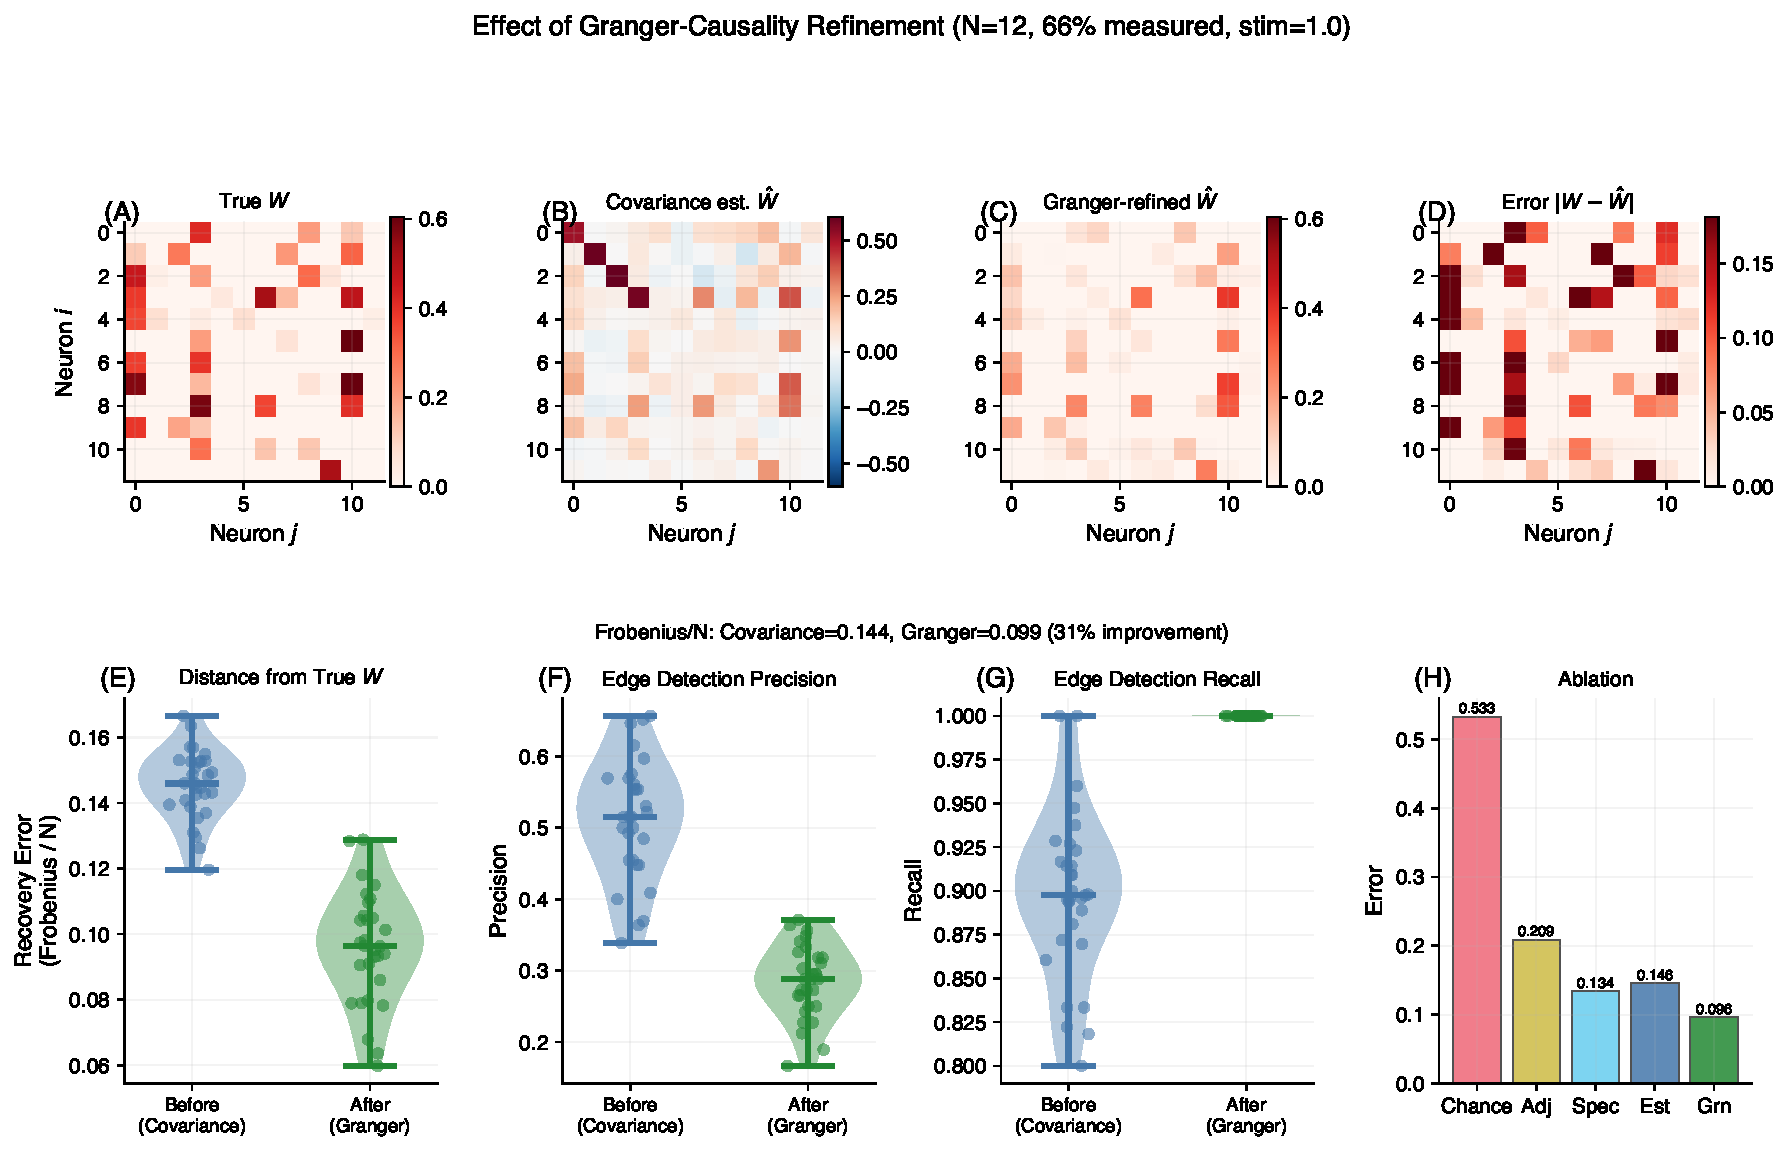
\includegraphics[width=0.95\linewidth]{figures/fig4_granger_refinement.pdf}
\\[3mm]
\large The Granger refinement step enforces biological constraints while preserving \textbf{all true edges} (perfect recall).
\end{tcolorbox}

\vspace{0.8cm}

% ── The Tradeoff ──
\begin{tcolorbox}[posterbox,title=The Experimenter's Dilemma]
\centering
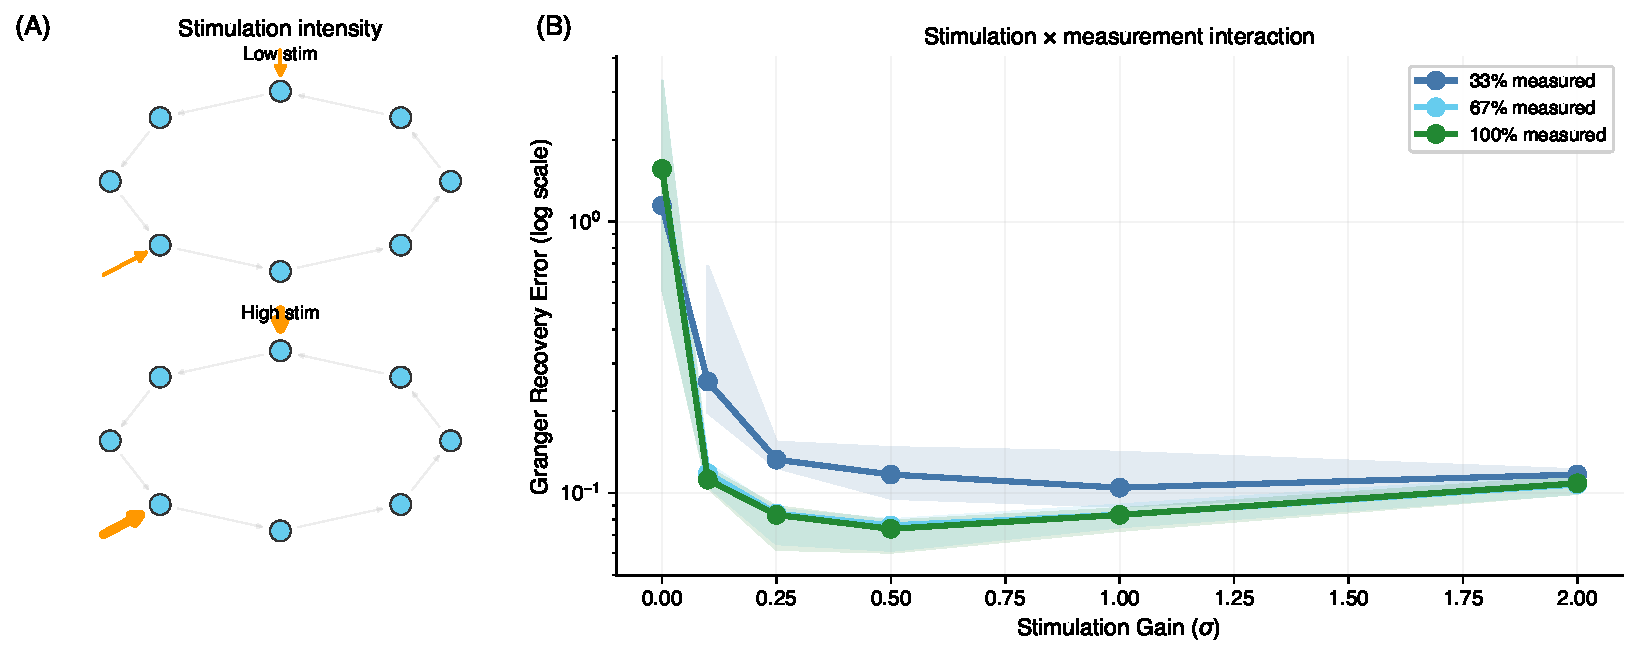
\includegraphics[width=0.95\linewidth]{figures/fig5_stimulation.pdf}
\\[3mm]
\large \textbf{Stimulation helps identification} --- but too much noise drowns the signal. The sweet spot: moderate intensity ($\sigma \approx 0.5$--$1.0$) on ${\sim}33\%$ of neurons.

\vspace{3mm}
Zero stimulation \emph{fails} at high measurement density because intrinsic dynamics alone don't excite all network modes.
\end{tcolorbox}

\vspace{0.8cm}

% ── Scaling ──
\begin{tcolorbox}[posterbox,title=Scales to Larger Networks]
\centering
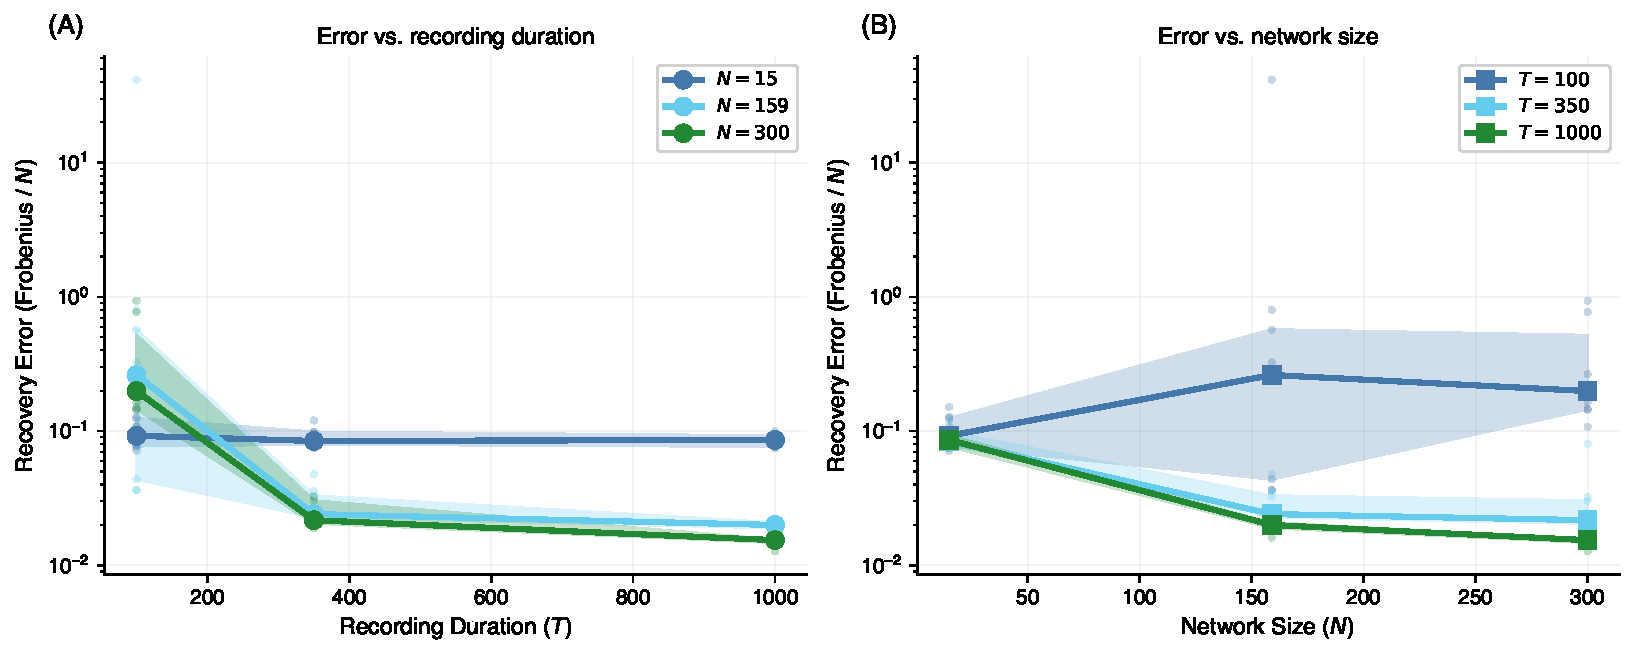
\includegraphics[width=0.95\linewidth]{figures/fig3_scaling.pdf}
\\[3mm]
\large Recovery improves with more neurons and longer recordings. At $N{=}30$, $T{=}1000$: error $0.050$ ($91\%$ over chance).
\end{tcolorbox}

\end{column}

% ════════════════════════════════════════════════════════════════════════════
% COLUMN 3 — Surprising Findings + Impact
% ════════════════════════════════════════════════════════════════════════════
\begin{column}{0.32\linewidth}

% ── The Surprise: Wrong Model Wins ──
\begin{tcolorbox}[posterbox,title=Surprise: The ``Wrong'' Model Wins,colframe=neuripsred,colbacktitle=neuripsred]
\centering
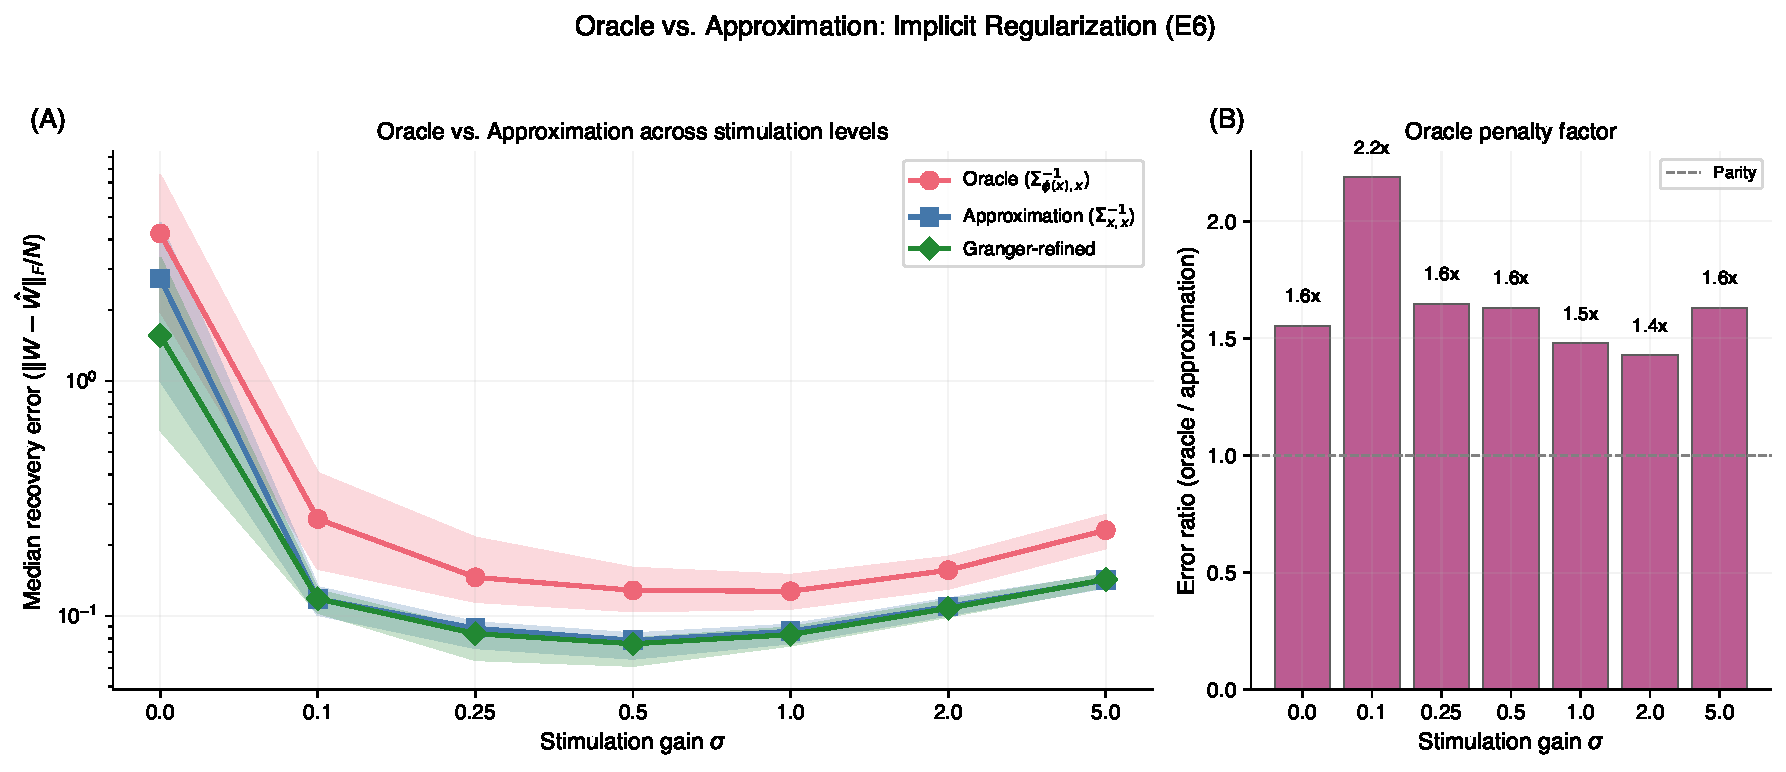
\includegraphics[width=0.95\linewidth]{figures/fig10_oracle_comparison.pdf}
\\[3mm]
\large The \textbf{linear approximation outperforms the oracle} that knows the true nonlinearity (up to $3.6\times$ worse for the oracle).

\vspace{3mm}
\textbf{Why?}\; The oracle must invert a \emph{worse-conditioned} matrix. The ``incorrect'' linear version trades bias for stability --- like ridge regression beating OLS.

\vspace{3mm}
{\color{neuripsred}\textbf{You don't need to characterize the neuronal transfer function.}}
\end{tcolorbox}

\vspace{0.8cm}

% ── Error Decomposition ──
\begin{tcolorbox}[posterbox,title=The Real Bottleneck]
\large
The linear approximation is \emph{not} the main error source. \textbf{Intrinsic CPG dynamics} are $3.1\times$ larger:

\vspace{3mm}
\begin{center}
\renewcommand{\arraystretch}{1.5}
\begin{tabular}{lcc}
  \toprule
  \textbf{Source} & \textbf{Error} & \textbf{Ratio} \\
  \midrule
  Model mismatch & $0.073$ & $1\times$ \\
  \rowcolor{neuripsred!15} CPG correlation & $0.229$ & $3.1\times$ \\
  \bottomrule
\end{tabular}
\end{center}

\vspace{3mm}
$\Rightarrow$ Future work: model the intrinsic dynamics, not the nonlinearity.
\end{tcolorbox}

\vspace{0.8cm}

% ── Takeaway ──
\begin{tcolorbox}[posterbox,title=For Experimentalists,colframe=neuripsgreen,colbacktitle=neuripsgreen]
\large
\begin{itemize}\setlength{\itemsep}{3pt}
  \item[\color{neuripsgreen}\textbf{1.}] Record $\geq 50\%$ of neurons per session
  \item[\color{neuripsgreen}\textbf{2.}] Stimulate $\sim 33\%$ at moderate intensity
  \item[\color{neuripsgreen}\textbf{3.}] Use the simple linear estimator --- it's \emph{better}
  \item[\color{neuripsgreen}\textbf{4.}] Run $\geq 50$ sessions for reliable coverage
\end{itemize}

\vspace{3mm}
\centering
{\small Code: \texttt{github.com/qsimeon/sparse\_matrix\_recovery}}
\end{tcolorbox}

\end{column}

\end{columns}

\end{frame}
\end{document}
